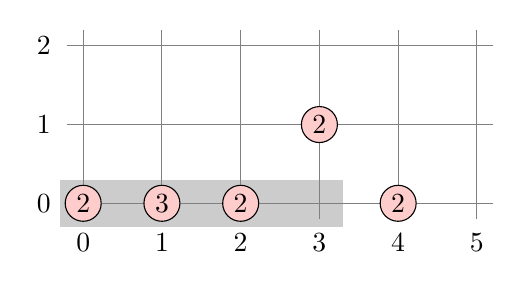
\begin{tikzpicture}
  \tikzstyle{vertex}=[draw, minimum size=13pt, inner sep=0pt]

  \fill[black!20!white] (-0.3, -0.3) -- (3.3, -0.3) -- (3.3, 0.3) -- (-0.3, 0.3) -- cycle;

  \foreach \x in {0, 1, ..., 5} {
    \draw[black!50!white] (\x, -0.2) -- (\x, 2.2);
    \node (x\x) at (\x, -0.5) {$\x$};
  }
  \foreach \y in {0, 1, 2} {
    \draw[black!50!white] (-0.2, \y) -- (5.2, \y);
    \node (y\y) at (-0.5, \y) {$\y$};
  }

  \node[vertex, circle, fill=red!20!white] (p1) at (0, 0) {$2$};
  \node[vertex, circle, fill=red!20!white] (p2) at (1, 0) {$3$};
  \node[vertex, circle, fill=red!20!white] (p3) at (2, 0) {$2$};
  \node[vertex, circle, fill=red!20!white] (p4) at (3, 1) {$2$};
  \node[vertex, circle, fill=red!20!white] (p5) at (4, 0) {$2$};
\end{tikzpicture}
